\documentclass{article}
\usepackage{v-test-paper}
\newenvironment{solution}{\par\noindent\color{red!85!black}$\Rightarrow$\vspace{0em}}{}
\title{\textsc{JEE Advanced 2012 Paper-II\\Physics}}
\date{}

\usepackage{mathtools}
\begin{document}
\maketitle
\begin{enumerate}
    
\item At time \( t = 0 \), terminal A in the circuit shown in the figure is connected to B by a key and an alternating current \( I(t) = I_0\cos(\omega t) \), with \( I_0 = 1 A \) and \( \omega = 500 \text{ rad s}^{-1} \) starts flowing in it with the initial direction shown in the figure. At \( t = \frac{7\pi}{6\omega} \), the key is switched from B to D. Now onwards only A and D are connected. A total charge \( Q \) flows from the battery to charge the capacitor fully. If \( C=20\mu F \), \( R=10 \Omega \) and the battery is ideal with \( emf \) of \( 50 V \), identify the correct statement(s).
    \begin{center}
        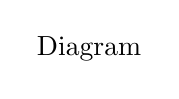
\begin{tikzpicture}
            \node at (0, 0) {Diagram};
        \end{tikzpicture}
    \end{center}
    \begin{tasks}(2)
        \task Magnitude of the maximum charge on the capacitor before \( t = \frac{7\pi}{6\omega} \) is \( 1 \times 10^{-3} C \).
        \task The current in the left part of the circuit just before \( t = \frac{7\pi}{6\omega} \) is clockwise.
        \task Immediately after A is connected to D, the current in \( R \) is \( 10 A \).
        \task \( Q = 2 \times 10^{-3} C \).
    \end{tasks}

    
\item A real gas behaves like an ideal gas if its
    \begin{tasks}(2)
        \task pressure and temperature are both high
        \task pressure and temperature are both low
        \task pressure is high and temperature is low
        \task pressure is low and temperature is high\ans
    \end{tasks}

    
\item A car starts moving rectilinearly, first with acceleration $w = -5.0\ m/s^2$ (the initial velocity is equal to zero), then uniformly, and finally, decelerating at the same rate $w$, comes to a stop. The total time of motion equals $\tau = 25\ s$. The average velocity during that time is equal to $\langle v \rangle = 72\ km$ per hour. How long does the car move uniformly?

    \item Given below are two statements:\\
\textbf{Statement I}: An elevator can go up or down with uniform speed when its weight is balanced with the tension of its cable.

\textbf{Statement II}: Force exerted by the floor of an elevator on the foot of a person standing on it is more than his/her weight when the elevator goes down with increasing speed.

In the light of the above statements, choose the correct answer from the options given below:
\begin{tasks}(1)
    \task Statement I is false but Statement II is true
    \task Both Statement I and Statement II are true
    \task Both Statement I and Statement II are false
    \task Statement I is true but Statement II is false
\end{tasks}
    
\item A point source $S$ is placed at the bottom of a transparent block of height $10\ mm$ and refractive index $2.72$. It is immersed in a lower refractive index liquid as shown in the figure. It is found that the light emerging from the block to the liquid forms a circular bright spot of diameter $11.54\ mm$ on the top of the block. The refractive index of the liquid is
    \begin{center}
        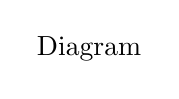
\begin{tikzpicture}
            \node at (0, 0) {Diagram};
            % Note: The actual diagram should replace this placeholder
        \end{tikzpicture}
    \end{center}
    \begin{tasks}(2)
        \task \(1.21\)
        \task \(1.30\)
        \task \(1.36\)
        \task \(1.42\)
    \end{tasks}

    
\item Consider a disc rotating in the horizontal plane with a constant angular speed $\omega$ about its centre $O$. The disc has a shaded region on one side of the diameter and an unshaded region on the other side as shown in the figure. When the disc is in the orientation as shown, two pebbles $P$ and $Q$ are simultaneously projected at an angle towards $R$. The velocity of projection is in the $y$-$z$ plane and is same for both pebbles with respect to the disc. Assume that (i) they land back on the disc before the disc has completed $\frac{1}{8}$ rotation, (ii) their range is less than half the disc radius, and (iii) $\omega$ remains constant throughout. Then
    \begin{center}
        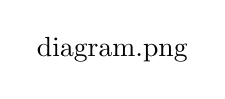
\begin{tikzpicture}
            \node at (0, 0) {diagram.png};
        \end{tikzpicture}
    \end{center}
    \begin{tasks}(1)
        \task $P$ lands in the shaded region and $Q$ in the unshaded region.
        \task $P$ lands in the unshaded region and $Q$ in the shaded region.
        \task Both $P$ and $Q$ land in the unshaded region.
        \task Both $P$ and $Q$ land in the shaded region.
    \end{tasks}

    \item Ratio of thermal energy released in two resistors \(R\) and \(3R\) connected in parallel in an electric circuit is :
\begin{tasks}(2)
    \task \(1 : 1\)
    \task \(1 : 27\)
    \task \(1 : 3\)
    \task \(3 : 1\)
\end{tasks}
    
\item A spherical metal shell A of radius $R_A$ and a solid metal sphere B of radius $R_B$ ($R_B < R_A$) are kept far apart and each is given charge $`+Q'$. Now they are connected by a thin metal wire. Then
    \begin{tasks}(2)
        \task $E_{\text{inside}}^A = 0$
        \task $Q_A > Q_B$
        \task $\frac{\sigma_A}{\sigma_B} = \frac{R_B}{R_A}$
        \task $E_{\text{on surface}}^A < E_{\text{on surface}}^B$
    \end{tasks}

    

\begin{center}
    \textsc{Paragraph for Questions 9 and 10}
\end{center}

Most materials have the refractive index, \( n > 1 \). So, when a light ray from air enters a naturally occurring material, then by Snell's law, \(\frac{\sin \theta_1}{\sin \theta_2} = \frac{n_2}{n_1}\), it is understood that the refracted ray bends towards the normal. But it never emerges on the same side of the normal as the incident ray. According to electromagnetism, the refractive index of the medium is given by the relation, \(n = \left( \frac{c}{v} \right) = \sqrt{\epsilon_r \mu_r}\), where \(c\) is the speed of electromagnetic waves in vacuum, \(v\) its speed in the medium, \(\epsilon_r\) the relative permittivity and \(\mu_r\) the permeability of the medium respectively.

In normal materials, both \(\epsilon_r\) and \(\mu_r\) are positive, implying positive \(n\) for the medium. When both \(\epsilon_r\) and \(\mu_r\) are negative, one must choose the negative root of \(n\). Such negative refractive index materials can now be artificially prepared and are called meta-materials. They exhibit significantly different optical behavior, without violating any physical laws. Since \(n\) is negative, it results in a change in the direction of propagation of the refracted light. However, similar to normal materials, the frequency of light remains unchanged upon refraction even in meta-materials.

\begin{center}
    \begin{tikzpicture}
        % As I cannot replicate the exact diagrams from the image, I'll draw a simple representation
        % Diagram A
        \draw (-4,0) -- (0,0); % Surface line
        \draw[-stealth] (-3,-1) -- (-2,0); % Incident ray
        \draw[dashed] (-2,0) -- (-2,1); % Normal line
        \draw[-stealth] (-2,0) -- (-1,0.5); % Refracted ray diagram A
        
        % Diagram B (similar to A, mirrored vertically)
        \draw (0,0) -- (4,0); % Surface line
        \draw[-stealth] (1,-1) -- (2,0); % Incident ray
        \draw[dashed] (2,0) -- (2,1); % Normal line
        \draw[-stealth] (2,0) -- (3,-0.5); % Refracted ray diagram B
        
        \node at (-2,-1.5) {(A)};
        \node at (2,-1.5) {(B)};
        
        % As the actual diagrams also include (C) and (D), extend as needed
        % Nodes can represent the diagrams' labels
        
    \end{tikzpicture}
\end{center} 

\item For light incident from air on a meta-material, the appropriate ray diagram is
    \begin{tasks}(2)
        \task Diagram A
        \task Diagram B
        \task Diagram C
        \task Diagram D
    \end{tasks} 

\item Choose the correct statement.
    \begin{tasks}(1)
        \task The speed of light in the meta-material is \( v = \frac{c}{|n|} \)
        \task The speed of light in the meta-material is \( v = \frac{c}{n} \)
        \task The speed of light in the meta-material is \( v = c \)
        \task The wavelength of the light in the meta-material \( \lambda_m \) is given by \( \lambda_m = \lambda_{\text{air}}|n|\), where \( \lambda_{\text{air}} \) is the wavelength of the light in air.
    \end{tasks} 

    
\begin{center}
    \textsc{Paragraph For Questions 11 \& 12}
\end{center}

In the figure a container is shown to have a movable (without friction) piston on top. The container and the piston are all made of perfectly insulating material allowing no heat transfer between outside and inside the container. The container is divided into two compartments by a rigid partition made of a thermally conducting material that allows slow transfer of heat. The lower compartment of the container is filled with 2 moles of an ideal monatomic gas at 700 K and the upper compartment is filled with 2 moles of an ideal diatomic gas at 400 K. The heat capacities per mole of an ideal monatomic gas are $C_V = \dfrac{3}{2} R, C_p = \dfrac{5}{2} R$, and those for an ideal diatomic gas are $C_V = \dfrac{5}{2} R,C_p = \dfrac{7}{2} R$.

\begin{center}
    \begin{tikzpicture}
        % Define the style for the piston
        \tikzset{piston/.style={thick}}
        % Draw the container
        \draw[piston] (0,0) -- (0,3) -- (2,3) -- (2,0) -- cycle;
        % Draw the partition
        \draw[piston] (0,1.5) -- (2,1.5);
        % Draw the piston
        \draw[piston, pattern=north east lines] (0,3) rectangle (2,3.25);
        % Label partition
        \draw[-stealth] (2.25,1.5) -- node[right] {Partition} ++(0,1);
        % Label lower gas
        \node at (1,0.75) {700 K};
        % Label upper gas
        \node at (1,2.25) {400 K};
    \end{tikzpicture}
\end{center} 

\item Consider the partition to be rigidly fixed so that it does not move. When equilibrium is achieved, the final temperature of the gases will be
    \begin{tasks}(4)
        \task 550 K
        \task 525 K
        \task 513 K
        \task 490 K
    \end{tasks}

    \begin{solution}
        \begin{align*}
            \intertext{Let's assume the final temperature of the gases to be $T_f$ at equilibrium.}
            \intertext{As the container is perfectly insulated, heat exchange must be zero.}
            \Delta Q_{\textit{lower compartment}} + \Delta Q_{\textit{upper compartment}} &= 0\\
            \intertext{Lower compartment will exchange heat at constant volume and upper compartment at constant pressure.}
            nC_v \Delta T + n C_p \Delta T &=0\\ 
            2 \left(\dfrac{3}{2} R\right) (T_f-700) + 2 \left(\dfrac{7}{2} R\right) (T_f - 400) &= 0\\
            3(T_f - 700) + 7(T_f - 400) &= 0\\
            3T_f - 2100 + 7T_f - 2800 &= 0\\
            10T_f &= 4900\\
            \Rightarrow T_f &= 490 \text{ K}
            \intertext{Thus, the final temperature of the gases at equilibrium will be 490 K.}
            \intertext{The correct option is (d).}
        \end{align*}
    \end{solution}
    
    

\item Now consider the partition to be free to move without friction so that the pressure of gases in both compartments is the same. Then total work done by the gases till the time they achieve equilibrium will be
    \begin{tasks}(4)
        \task 250 R
        \task 200 R
        \task 100 R
        \task $-100$ R
    \end{tasks} 

    \begin{solution}
        \begin{align*}
            \intertext{Now, consider the partition to be free to move resulting in equal pressures on both compartments at equilibrium.}
            \intertext{Again, total heat exchange must be zero.}
            \Delta Q_{\textit{lower compartment}} + \Delta Q_{\textit{upper compartment}} &= 0\\
            \intertext{This time both compartments will exchange heat at constant pressure.}
            nC_p \Delta T + n C_p \Delta T &=0\\
            2 \left(\dfrac{5}{2} R\right) (T_f-700) + 2 \left(\dfrac{7}{2} R\right) (T_f - 400) &= 0\\
            5(T_f - 700) + 7(T_f - 400) &= 0\\
            5T_f - 3500 + 7T_f - 2800 &= 0\\
            12T_f &= 6300\\
            \Rightarrow T_f &= 525 \text{ K}
            \intertext{Thus, the final temperature of the gases at equilibrium will be 525 K.}
            \intertext{Now, let's calculate the total work done by the gases.}
            \intertext{The work done by the lower compartment will be}
            Q_{\textit{system}} &= W_{\textit{system}} + \Delta U_{\textit{system}}\\
            0 &= W_{\textit{system}} + \Delta U_{\textit{lower compartment}} + \Delta U_{\textit{upper compartment}}\\
            W_{\textit{system}} &= -\left(nC_v \Delta T + nC_v \Delta T\right)\\
            &= -2 \left(\dfrac{3}{2} R\right) (525 - 700) - 2 \left(\dfrac{5}{2} R\right) (525 - 400)\\
            &= -3 R (-175) - 5 R (125)\\
            &= 525 R - 625 R\\
            &= -100 R
            \intertext{Thus, the total work done by the gases till the time they achieve equilibrium will be $-100 R$.}
            \intertext{The correct option is (d).}
        \end{align*}
    \end{solution}

    \begin{center}
    \textsc{Paragraph for Questions 13 and 14}
\end{center}

A small block of mass 1 kg is released from rest at the top of a rough track. The track is a circular arc of radius 40 m. The block slides along the track without toppling and a frictional force acts on it in the direction opposite to the instantaneous velocity. The work done in overcoming the friction up to the point \( Q \), as shown in the figure below, is 150 J. (Take the acceleration due to gravity, \( g = 10\ m/s^2 \)).

\begin{center}
    \begin{tikzpicture}
        % Track
        \draw[thick] (0,0) arc (180:240:2cm);
        % Block sliding marks
        \draw[dashed] (0,0) -- (1.73, -1); % Extended line that fades
        % Radius lines
        \draw[dashed] (0,0) -- (-2,0) node[midway, above] {\( R \)};
        \draw[dashed] (1.73, -1) -- (0,0) node[midway, above right] {\( R \)};
        % Angle
        \draw (0,-0.5) arc (270:300:0.5cm) node[midway, right] {\( 30^\circ \)};
        % Point labels
        \filldraw[black] (0,0) circle (2pt) node[above left] {\( P \)};
        \filldraw[black] (1.73, -1) circle (2pt) node[below right] {\( Q \)};
        % Axis labels
        \draw[->] (-2.5,0) -- (2.5,0) node[right] {\( x \)};
        \draw[->] (0,0) -- (0,2.5) node[above] {\( y \)};
    \end{tikzpicture}
\end{center}

\item The speed of the block when it reaches the point \( Q \) is
    \begin{tasks}(4)
        \task \( 5\ m/s^{-1} \)
        \task \( 10\ m/s^{-1} \)
        \task \( 10\sqrt{3}\ m/s^{-1} \)
        \task \( 20\ m/s^{-1} \)
    \end{tasks}
    
\item The magnitude of the normal reaction that acts on the block at the point \( Q \) is
    \begin{tasks}(4)
        \task \( 7.5\ N \)
        \task \( 8.6\ N \)
        \task \( 11.5\ N \)
        \task \( 22.5\ N \)
    \end{tasks}
    
\item In the given circuit, the AC source has $\omega = 100\ \text{rad/s}$. Considering the inductor and capacitor to be ideal, the correct choice(s) is(are)
    \begin{center}
        \begin{circuitikz}[american]
            \draw (0,0)
            to[V, V=$20\ V$] (0,2) % The voltage source
            to[L, L=$0.5\ H$] (2,2) % The inductor
            to[C, C=$100\ \mu F$] (4,2) % The capacitor
            to[R, R=$100\ \Omega$] (4,0) % 100 ohm resistor
            -- (0,0);
            \draw (2,2)
            to[R, R=$50\ \Omega$] (2,0); % 50 ohm resistor
        \end{circuitikz}
    \end{center}
    \begin{tasks}(1)
        \task The current through the circuit, $I$ is $0.3\ A$.
        \task The current through the circuit, $I$ is $0.3\sqrt{2}\ A$.
        \task The voltage across $100\ \Omega$ resistor is $10\sqrt{2}\ V$.
        \task The voltage across $50\ \Omega$ resistor is $10\ V$.
    \end{tasks}

    \item A planet of mass \( M \), has two natural satellites with masses \( m_1 \) and \( m_2 \). The radii of their circular orbits are \( R_1 \) and \( R_2 \) respectively. Ignore the gravitational force between the satellites. Define \( v_1 \), \( L_1 \), \( K_1 \) and \( T_1 \) to be, respectively, the orbital speed, angular momentum, kinetic energy and time period of revolution of satellite 1; and \( v_2 \), \( L_2 \), \( K_2 \) and \( T_2 \) to be the corresponding quantities of satellite 2. Given \( m_1/m_2 = 2 \) and \( R_1/R_2 = 1/4 \), match the ratios in List-I to the numbers in List-II.

\begin{center}
    \renewcommand{\arraystretch}{2.5}
    \begin{table}
        \centering
        \begin{tabular}{p{0.25cm}p{6cm}|p{0.25cm}p{6cm}}
        \hline
        & List-I & &List-II \\
        \hline
        P. & \( \frac{v_1}{v_2} \) & 1. & \( \frac{1}{8} \) \\
        Q. & \( \frac{L_1}{L_2} \) & 2. & \( 1 \) \\
        R. & \( \frac{K_1}{K_2} \) & 3. & \( 2 \) \\
        S. & \( \frac{T_1}{T_2} \) & 4. & \( 8 \) \\
        \hline
        \end{tabular}
    \end{table}
\end{center}

\begin{tasks}(2)
    \task \( P \rightarrow 4; \) \( Q \rightarrow 2; \) \( R \rightarrow 1; \) \( S \rightarrow 3 \)
    \task \( P \rightarrow 3; \) \( Q \rightarrow 2; \) \( R \rightarrow 4; \) \( S \rightarrow 1 \)
    \task \( P \rightarrow 2; \) \( Q \rightarrow 3; \) \( R \rightarrow 1; \) \( S \rightarrow 4 \)
    \task \( P \rightarrow 2; \) \( Q \rightarrow 3; \) \( R \rightarrow 4; \) \( S \rightarrow 1 \)
\end{tasks}

\begin{solution}
    Since the satellites are in circular orbits, we can use the following equations governing their motion:
    \begin{align*}
        v &= \sqrt{\frac{GM}{R}} \quad \text{(Orbital speed)} \\
        L &= mRv \quad \text{(Angular momentum)} \\
        K &= \frac{1}{2}mv^2 \quad \text{(Kinetic energy)} \\
        T &= \frac{2\pi R}{v} \quad \text{(Time period)}
    \end{align*}
    where \( G \) is the gravitational constant.
    \begin{align*}
        \intertext{For the ratio \( P = \frac{v_1}{v_2} \), we use the orbital speed equation:}
        v_1 &= \sqrt{\frac{GM}{R_1}} \\
        v_2 &= \sqrt{\frac{GM}{R_2}} \\
        \frac{v_1}{v_2} &= \sqrt{\frac{R_2}{R_1}} = \sqrt{\frac{4}{1}} = 2 \quad \Rightarrow P \rightarrow 3.
        \intertext{For the ratio \( Q = \frac{L_1}{L_2} \), we use the angular momentum equation:}
        L_1 &= m_1R_1v_1 \\
        L_2 &= m_2R_2v_2 \\
        \frac{L_1}{L_2} &= \frac{m_1R_1}{m_2R_2}\frac{v_1}{v_2} = \frac{2}{1}\frac{1}{4}\cdot2 = \frac{1}{1} = 1 \quad \Rightarrow Q \rightarrow 2.
        \intertext{For the ratio \( R = \frac{K_1}{K_2} \), we use the kinetic energy equation:}
        K_1 &= \frac{1}{2}m_1v_1^2 \\
        K_2 &= \frac{1}{2}m_2v_2^2 \\
        \frac{K_1}{K_2} &= \frac{m_1}{m_2}\left(\frac{v_1}{v_2}\right)^2 = \frac{2}{1}\cdot2^2 = 8 \quad \Rightarrow R \rightarrow 4.
        \intertext{Finally, for the ratio \( S = \frac{T_1}{T_2} \), we use the time period equation:}
        T_1 &= \frac{2\pi R_1}{v_1} \\
        T_2 &= \frac{2\pi R_2}{v_2} \\
        \frac{T_1}{T_2} &= \frac{R_1}{R_2}\frac{v_2}{v_1} = \frac{1}{4}\cdot\frac{1}{2} = \frac{1}{8} \quad \Rightarrow S \rightarrow 1.
    \end{align*}
    Thus, we have P matching with 3, Q with 2, R with 4, and S with 1. The final answer is
    \begin{align*}
        P \rightarrow 3; \quad Q \rightarrow 2; \quad R \rightarrow 4; \quad S \rightarrow 1.\\
        \intertext{Therefore, option (b) is correct.}
    \end{align*}
\end{solution}
    \item Match List I with List II and select the correct answer using the codes given below the lists:

\begin{center}
    \renewcommand{\arraystretch}{2}
    \begin{table}[h]
        \centering
        \begin{tabular}{p{0.25cm}p{8cm}|p{0.25cm}p{5cm}}
        \hline
        & List I & & List II \\
        \hline
        (P)& Boltzmann constant & (1) & $[ML^2T^{-1}]$ \\
        (Q)& Coefficient of viscosity & (2) & $[ML^{-1}T^{-1}]$ \\
        (R)& Planck constant & (3) & $[MLT^{-3}K^{-1}]$ \\
        (S)& Thermal conductivity & (4) & $[ML^2T^{-2}K^{-1}]$ \\
        \hline
        \end{tabular}
    \end{table}
\end{center}

\begin{tasks}(2)
    \task $P \rightarrow 3$, $Q \rightarrow 1$, $R \rightarrow 2$, $S \rightarrow 4$
    \task $P \rightarrow 3$, $Q \rightarrow 2$, $R \rightarrow 1$, $S \rightarrow 4$
    \task $P \rightarrow 4$, $Q \rightarrow 2$, $R \rightarrow 1$, $S \rightarrow 3$
    \task $P \rightarrow 4$, $Q \rightarrow 1$, $R \rightarrow 2$, $S \rightarrow 3$
\end{tasks}
    
\begin{enumerate}
    \item A container with 1 kg of water in it is kept in sunlight, which causes the water to get warmer than the surroundings. The average energy per unit time per unit area received due to the sunlight is 700 Wm$^{-2}$ and it is absorbed by the water over an effective area of 0.05 m$^2$. Assuming that the heat loss from the water to the surroundings is governed by Newton’s law of cooling, the difference (in $^\circ$C) in the temperature of water and the surroundings after a long time will be \underline{\hspace{3cm}}. (Ignore effect of the container, and take constant for Newton’s law of cooling = 0.001 s$^{-1}$, Heat capacity of water = 4200 J kg$^{-1}$ K$^{-1}$)
\end{enumerate}

    
\item The focal length of a thin biconvex lens is \(20\text{cm}\). When an object is moved from a distance of \(25\text{cm}\) in front of it to \(50\text{cm}\), the magnification of its image changes from \(m_{25}\) to \(m_{50}\). The ratio \(\frac{m_{25}}{m_{50}}\) is \underline{\hspace{2.5cm}}.

    
\item An $\alpha$-particle and a proton are accelerated from rest by a potential difference of 100V. After this, their de Broglie wavelengths are $\lambda_\alpha$ and $\lambda_p$, respectively. The ratio $\frac{\lambda_p}{\lambda_\alpha}$, to the nearest integer, is \underline{\hspace{2.5cm}}.

\end{enumerate}
\end{document}